\documentclass[12pt]{article}

\textwidth=7.1in
\textheight=9.5in
\topmargin=-1in
\headheight=0.3in
\headsep=0.2in
\hoffset=-0.6in

\usepackage[section]{placeins}
\usepackage{float}
\usepackage{datetime}
\usepackage{color}
\usepackage{graphicx}
\usepackage{epstopdf}
\usepackage{subcaption}
\usepackage[labelfont=bf]{caption}
\usepackage{placeins}
\usepackage[hidelinks]{hyperref}

\usepackage{chngcntr}
\counterwithin{figure}{section}


\title{NMRLipids Project on Polarizable Lipid Force Fields}

\begin{document}

\maketitle

\section{Introduction}
%\date{\today}
So far, the NMRLipids community has focused on the performance of non-polarizable lipid force fields and we have not included a study on the polarizable
models. As the inclusion of polarizability, both implicitly and explicitly, is getting more popular, I think a systematic review and benchmark study of the polarizable force fields would be very useful for the entire community. At this moment, the idea is to focus only on the explicit polarization.\\

Recently there has been a \underline{NMRLipids (http://nmrlipids.blogspot.fi/2018/04/new-nmrlipids-related-publication.html) based} publication by \underline{Josef Melcr~\textit{et al.}} (http://dx.doi.org/10.1021/acs.jpcb.7b12510) where they included the electronic polarizability \textit{implicitly}. Their results showed a great improvement on the calculated order parameters in response to the added CaCl$_{2}$. This suggests that including polarizability, even implicitly, can significantly improve performance.\\

At the moment, there are three main polarizable lipid force fields with explicit electronic polarization: CHARMM-Drude~\cite{li2017drude}, AMOEBA~\cite{chu2018anionicpolarizable,chu2018polarizable}, and CHARMM-Fluctuating Charge (FQ)~\cite{lucas2012charge}. It is possible to obtain force field parameters and run them on GROMACS, AMBER, and CHARMM, respectively. Therefore, we need to have access to GROMACS, CHARMM, and AMBER MD engines unless someone ports all of these force fields to GROMACS.\\

In the following, I will try to give a glimpse of what is available and how well
is the performance of the aforementioned polarizable models. \\

\section{Available Literature}

In the CHARMM-Drude force field, which is based on the classical Drude oscillator, a
maximum-entropy method has been employed to match the experimental NMR order
parameters. As of today, cholesterol, DPPC, DMPC, DLPC, POPC, DOPC, DPPE, POPE, and DOPE
lipids have been parametrized. Furthermore, within the same force field there
are force field parameters for ions which we can further test. Fig.~\ref{fig:drudedppc} shows the NMR deuterium order parameters for the DPPC bilayer simulated by Li~\textit{et al.}~\cite{li2017drude} with the
CHARMM-Drude force field. One important observation is that they do not report
the sign of the order parameters. Second observation is that in the Drude force
field the order parameters have, overall, larger values compared to the original
C36 force field. The NMR order parameters for the POPC and POPE bilayers from the Drude polarizable force field are given in Figs.~\ref{fig:drudepopc}-\ref{fig:drudepope}. Please note that in all figures presented here, the full captions from the original publications are included as they are for convenience.\\

\begin{figure}[!hbt]
  \centering
  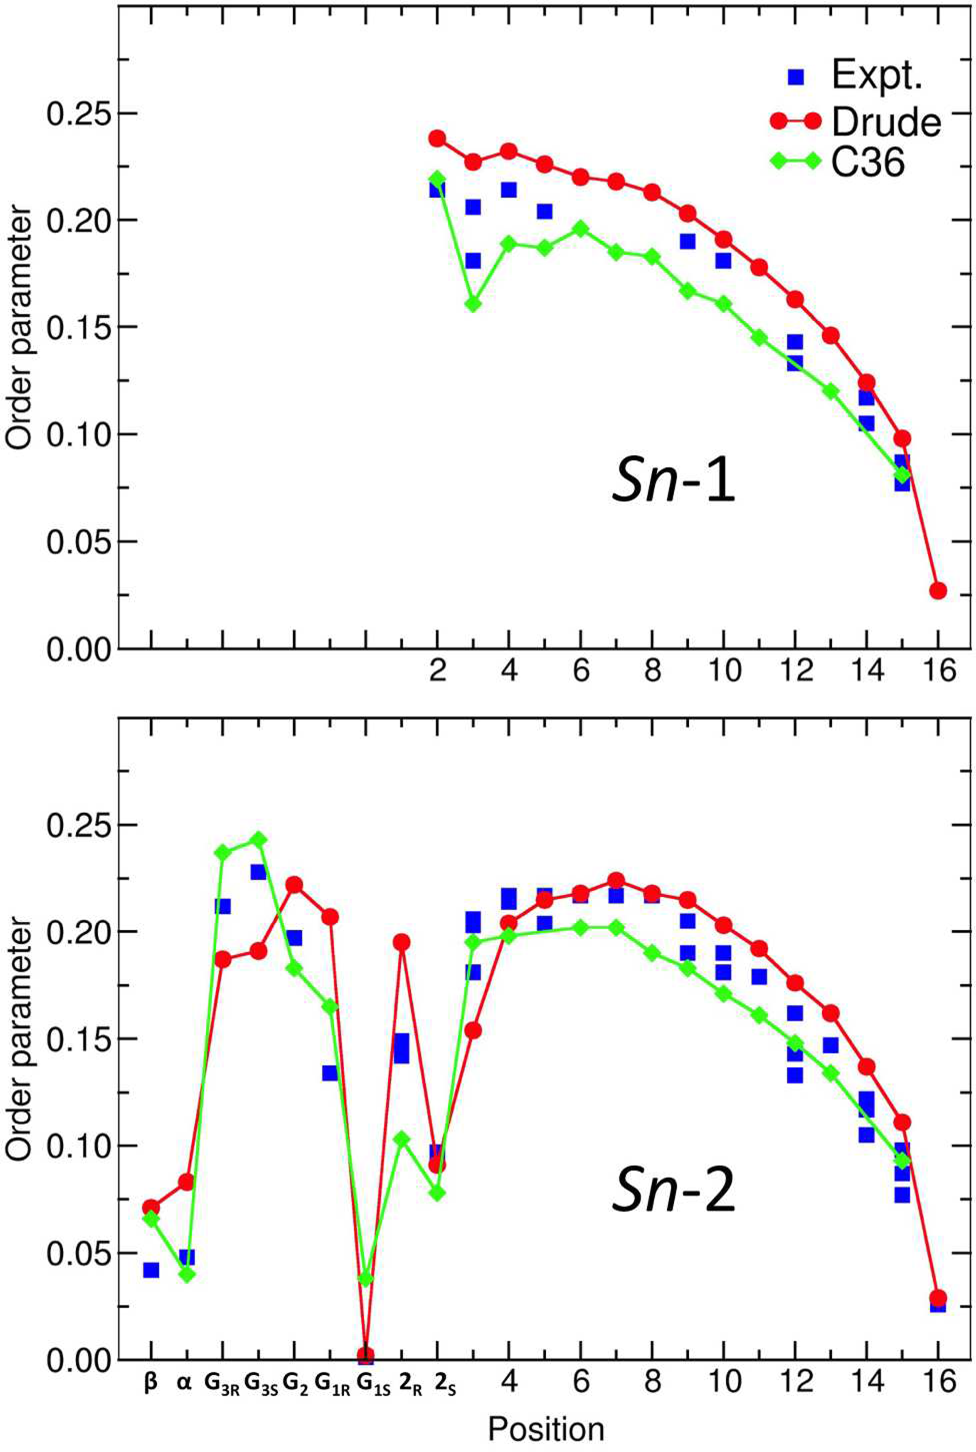
\includegraphics[width=0.4\textwidth]{../Figures/dppc_order_parameters_drude.png}
  \caption{NMR deuterium order parameter (SCD) values for a
  	hydrated DPPC bilayer from ~\cite{li2017drude}. Shown are the SCD calculated using the new
  	Drude polarizable force field (red), C36 additive force field (blue), and
  	measured from experiments (black). The results for the C36 force field
  	were taken from Klauda \textit{et al.}~\cite{klauda2010update}. Experimental data were taken from Seelig and co-workers~\cite{seelig1974dynamic,seelig1975bilayers,gally1975conformation,gally1981structure} and Strenk \textit{et al.}~\cite{strenk1985model}; the data for the Sn-2 chain is taken from Douliez and \textit{et al.}~\cite{douliez1995restatement}}
  \label{fig:drudedppc}
\end{figure}

\begin{figure}[!htb]
	\centering
	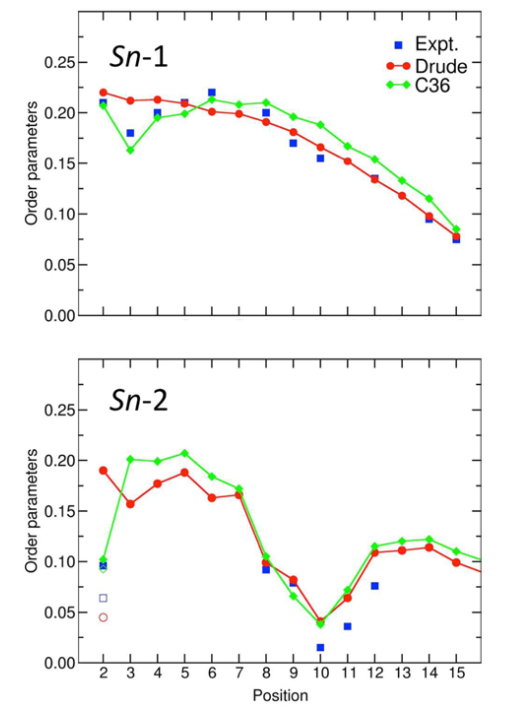
\includegraphics[width=0.4\textwidth]{../Figures/popc_order_parameters_drude.png}
	\caption{NMR deuterium order parameters (SCD) for a hydrated
		POPC bilayer from Drude polarizable force field~\cite{li2017drude}. Shown are the SCD calculated using the new Drude
		polarizable force field (red), C36 additive force field (blue), and
		measured from experiments (black). The results for the C36 force field were taken from Klauda \textit{et.al.}~\cite{klauda2010update}.The MD values were calculated at 303 K. The experimental data collected at 300 K is from Seelig and Seelig~\cite{seelig1975bilayers}.The open symbols at position 2 of the Sn-2 chain represent the split values of the order parameters for HR and HS.}
	\label{fig:drudepopc}
	\end{figure}
		
\begin{figure}[!hbt]
	\centering
	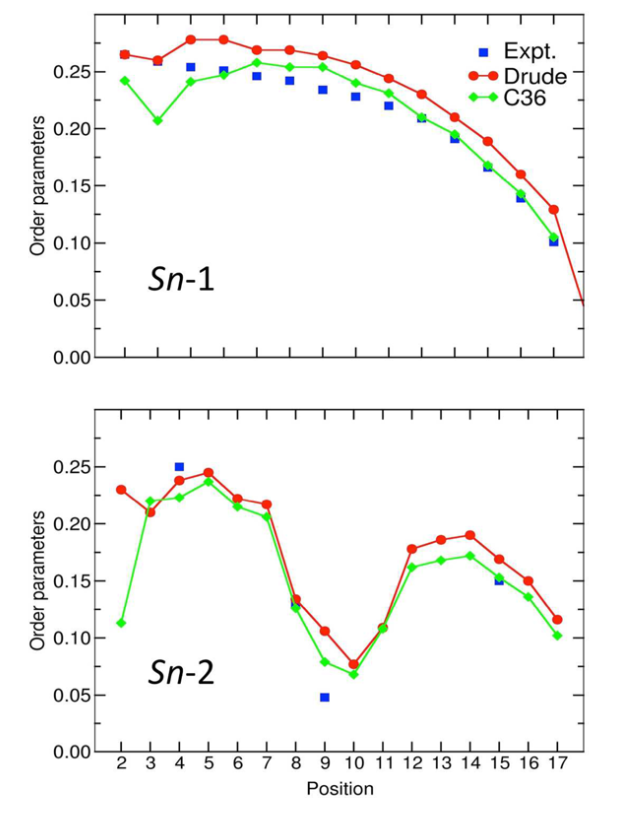
\includegraphics[width=0.4\textwidth]{../Figures/pope_order_parameters_drude.png}
	\caption{NMR deuterium order parameters (SCD ) for a hydrated POPE bilayer. Shown are the SCD calculated using the new Drude
		polarizable force field at 303 K (red), C36 additive force field at 310 K
		(blue), and measured from experiments at 310 K (black). The results for the C36 force field were taken from Klauda \textit{et al.}~\cite{klauda2010update}. The experimental data are taken from~\cite{shaikh2002monounsaturated,perly1985acyl}.}
	\label{fig:drudepope}
	\end{figure}
			
The Atomic Multipole Optimized Energetics for Biomolecular Applications (AMOEBA)
force field is based on representing the charge distribution of each atom by
atomic monopole, dipole, and quadrupole moments. The literature in this case a
bit scattered, but so far I managed to dig out force field parameters for DMPG~\cite{chu2018anionicpolarizable},
POPS~\cite{chu2018anionicpolarizable}, DOPC~\cite{chu2018polarizable}, and POPE~\cite{chu2018polarizable}. In the original paper the deuterium order
parameters have been reported without the signs and the reported experimental
values are sparse (Fig.~\ref{fig:amoebadopc}).\\

\begin{figure}[!hbt]
  \centering
  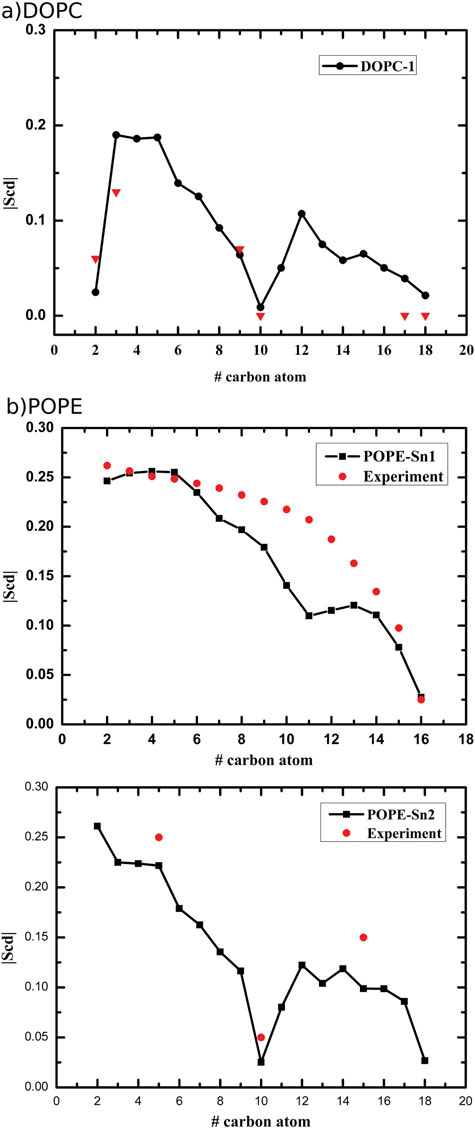
\includegraphics[width=0.4\textwidth]{../Figures/order_parameter_amoeba.png}
  \caption{NMR deuterium order parameters for DOPC and POPE lipids from AMOEBA
  force field~\cite{chu2018polarizable}.The order parameters for the DOPC and POPE bilayer system averaged over the last 20~ns simulations (a) Sn-1, (b) Sn-2, are compared with the experimental values that are shown in red~\cite{seelig1978molecular,perly1985acyl,shaikh2002monounsaturated}.}
\label{fig:amoebadopc}
\end{figure}

\begin{figure}[!hbt]
	\centering
	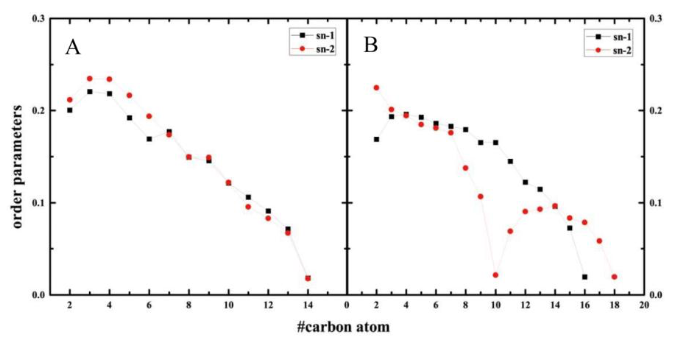
\includegraphics[width=0.4\textwidth]{../Figures/dmpg_pops_order_parameters_amoeba.png}
	\caption{The order parameters for bilayer system averaged over the last 20 ns simulations from the AMOEBA force field~\cite{chu2018anionicpolarizable}. (A) The
		order parameters for DMPG bilayer system; (B) The order parameters for POPS bilayer system. order parameters for DMPG bilayer system; (B) The order parameters for POPS bilayer system.}
	\label{fig:amoebadmpg}
\end{figure}

CHARMM-Fluctuating Charge/Charge equilibration (FQ/CHEQ, the name has changed a
few times over the course of development) force field allows the magnitude of
the individual atomic partial charges to change over the course of a simulation
by assigning a fictitious mass to each of the charges and treating them as
additional degrees of freedom in the equations of motion. So far, I managed to
find the force field parameters for DMPC~\cite{davis2009molecular} and DPPC~\cite{davis2009charge}, however a further work
on this force field, especially for the lipids, seems to be ceased. The order parameters reported in these papers are given in Figs.~\ref{fig:dmpccheq}-\ref{fig:dppccheq}\\

\begin{figure}[!hbt]
  \centering
  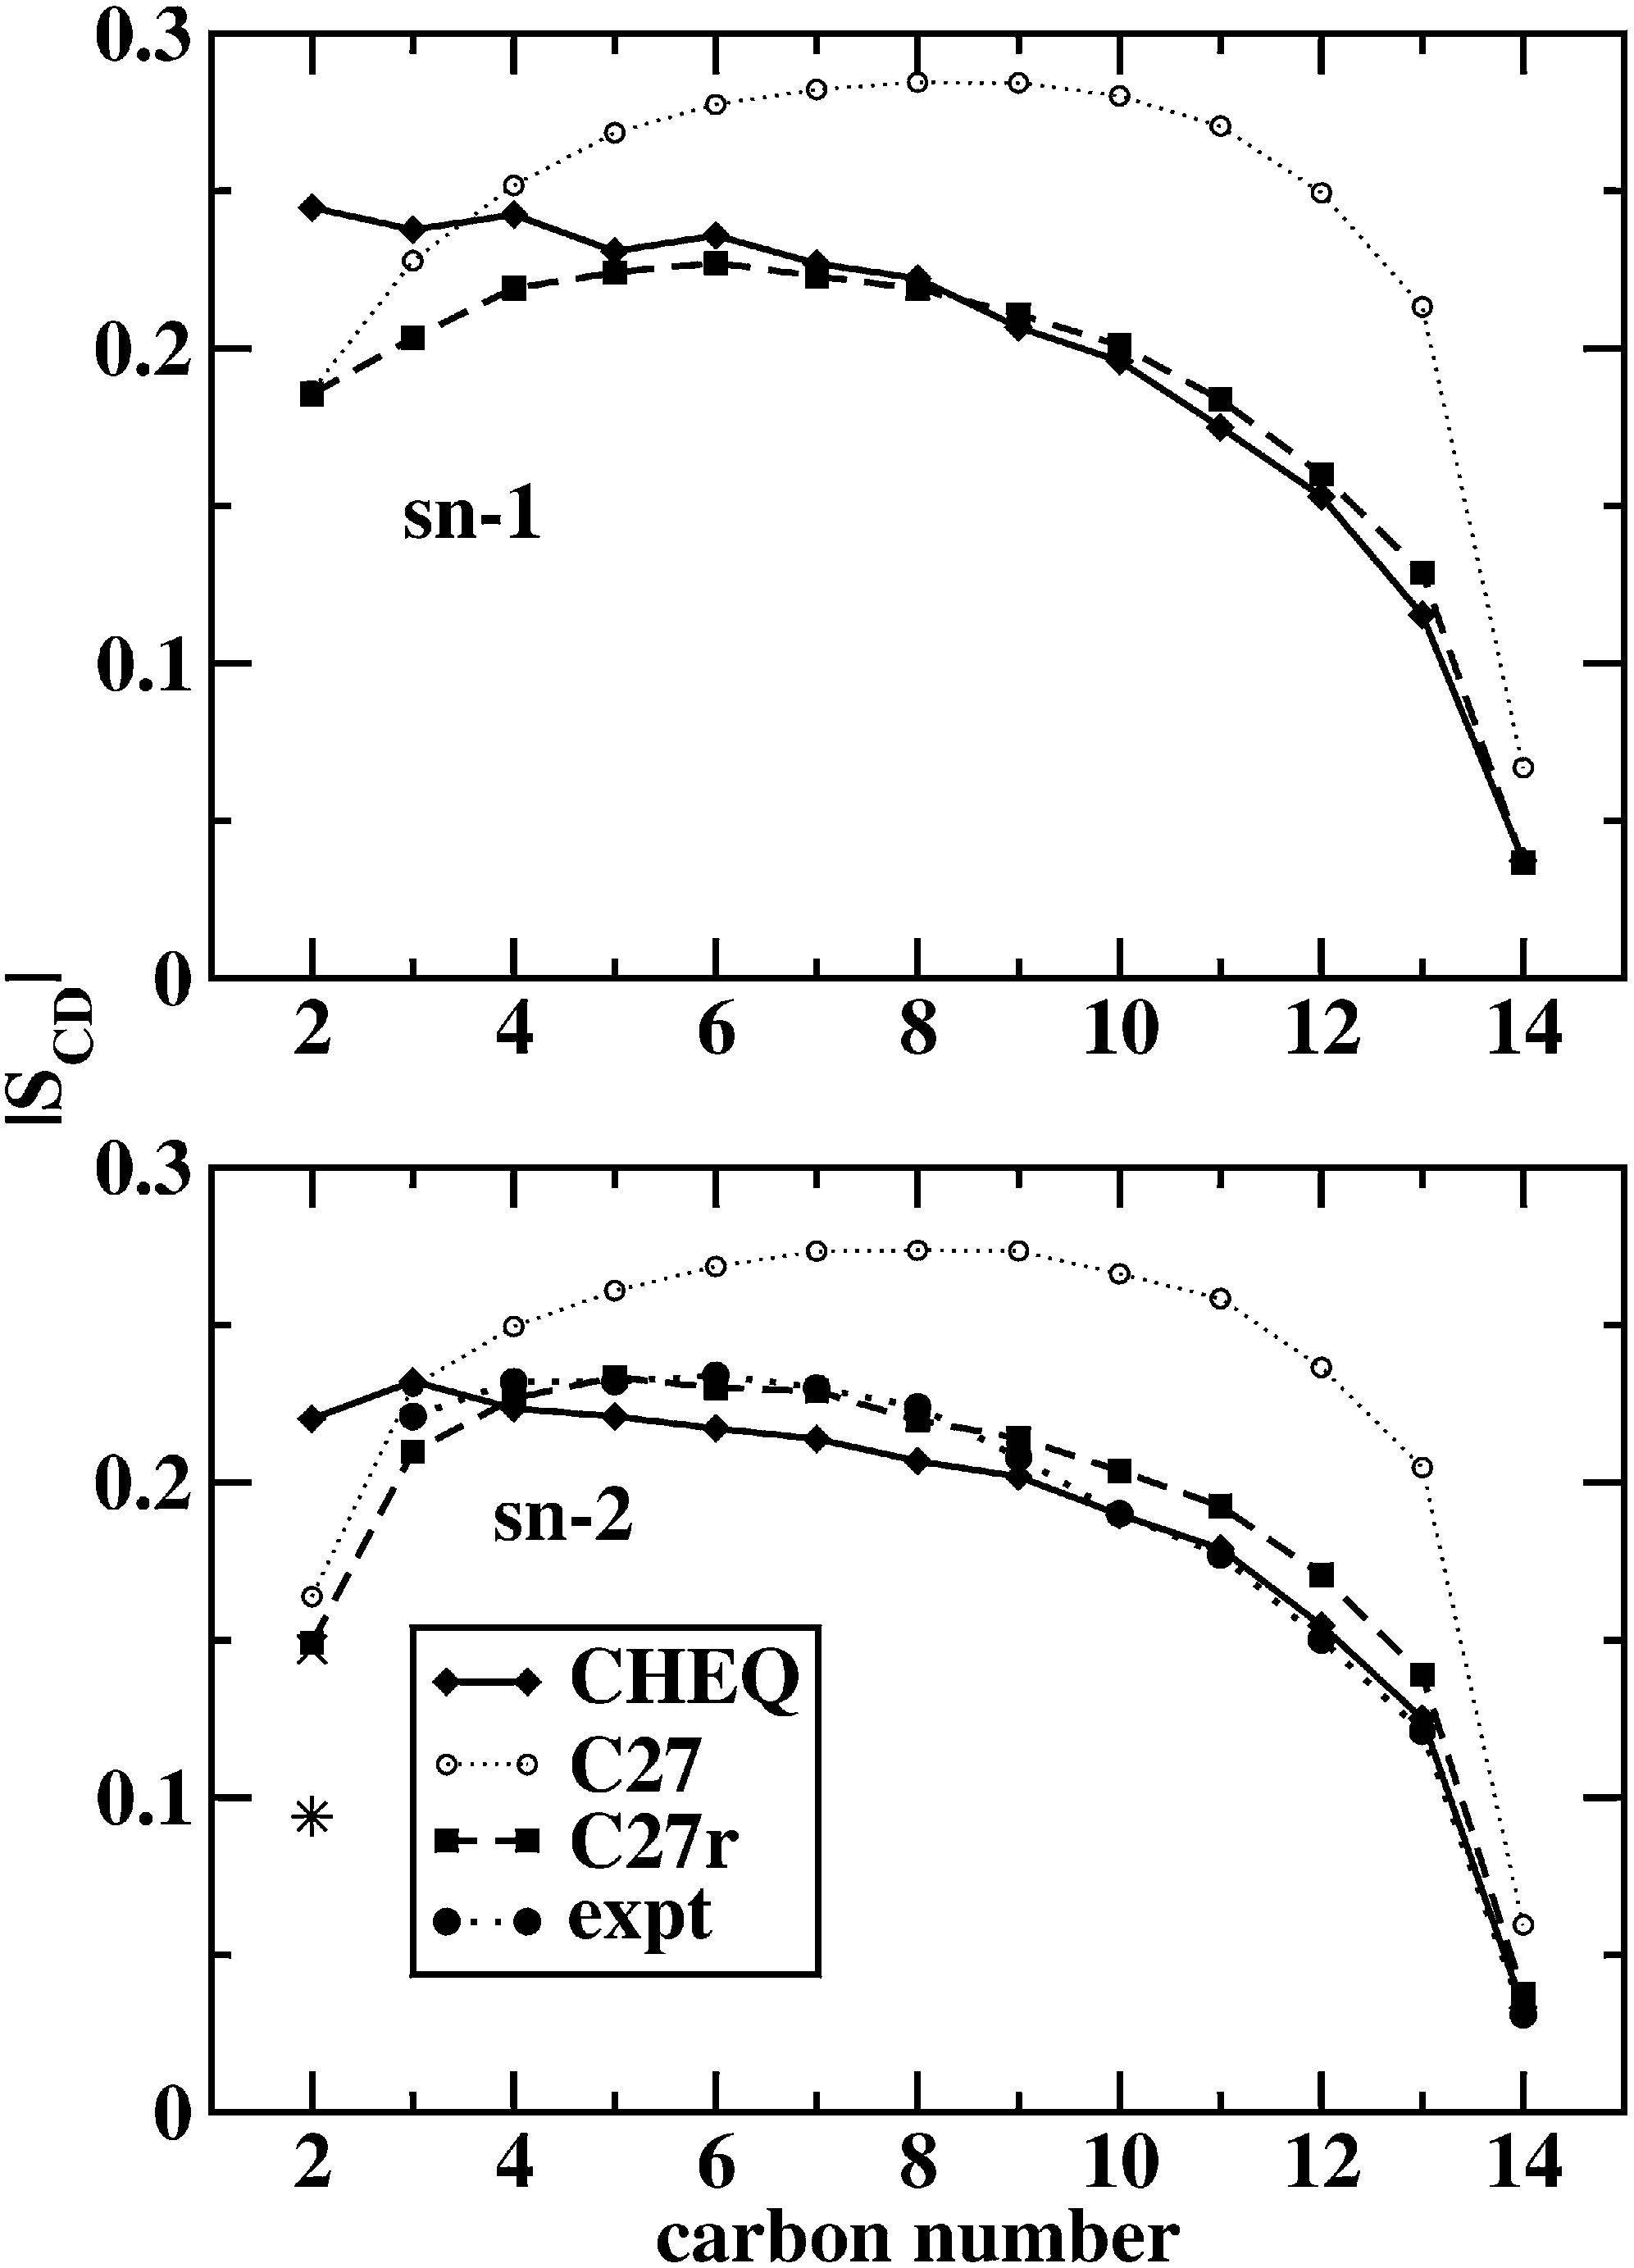
\includegraphics[width=0.4\textwidth]{../Figures/dmpc_order_charmmfq.png}
  \caption{Deuterium order parameters for the tail groups of DMPC as a function of position on the sn-1 (upper) and sn-2 (lower) hydrocarbon chain from CHEQ force field~\cite{davis2009molecular}. Values are shown for the polarizable (CHEQ) and nonpolarizable (C27) models, as well as for the revised CHARMM force field for alkanes (C27r)~\cite{klauda2005ab}. Experimental data~\cite{douliez1995restatement} for the asymmetric sn-2 chain (lower) are also shown, with the star and X symbols marking the values for the 2R and 2S hydrogens, respectively.}
  \label{fig:dmpccheq}
\end{figure}

\begin{figure}[!hbt]
	
	\centering
	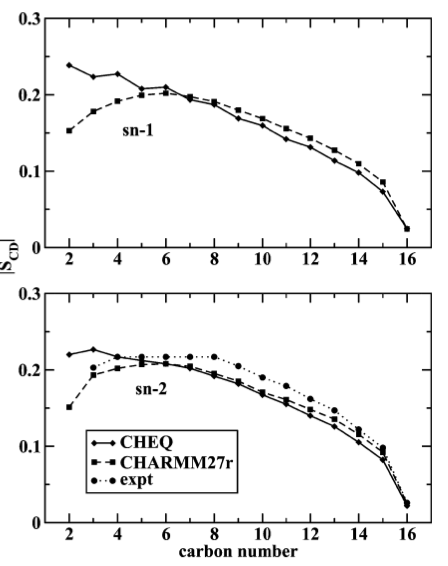
\includegraphics[width=0.4\textwidth]{../Figures/dppc_order_parameters_cheq.png}
	\caption{Magnitude of the deuterium order parameters for the tail groups as a function of position along the hydrocarbon chain for the DPPC from CHEQ force field~\cite{davis2009charge}. Values are shown for the polarizable CHEQ and nonpolarizable CHARMM27r models. Experimental data is also shown~\cite{douliez1995restatement}.}
	\label{fig:dppccheq}
	
\end{figure}

\section{Workflow and Data Contributions}
%Among the force fields I mentioned, CHARMM-Drude seems to be the
%most commonly and actively used. AMOEBA and CHARMM-FQ force fields have
%limited number of lipids in their databases, and particularly for the CHARMM-FQ
%it looks like no significant further work is done. Based on these, I would suggest us to focus mostly on the CHARMM-Drude and to use the data from the other force fields whene%ver they have the
%parameters.\\

Due to the limited number of force fields and available lipids, I would suggest
doing something similar to the NMRLipids II and IV projects combined: checking
the performance of all force fields for available zwitterionic and charged head
groups employing the NMR order parameters, X-ray form factors, ion binding, and correlation times. \\

%For the last year, as the NMRLipids community we have developed a Python script that performs the required calculations for the order parameters, X-ray form factors, and correlation times. Our current idea is to utilize this script and make it the main analysis source for this project. We are making the final touches to the script and we will make it available soon.\\

%Concerning the data contributions. We will be creating a public GitHub repository within the NMRLipids for this project. The Python script and its documentation/user guide will be available in this repository. We kindly ask everyone who are willing to contribute with their trajectories to upload them to the NMRLipids community on Zenodo. From there, you can analyse your trajectories using our Python script. Final step would be to upload the results, but not the trajectories, to the project's GitHub repository. Please comment under this post if you are willing to run/upload simulations.\\

In the meantime, I will be working on a literature review for the polarizable force fields that could reveal some other force fields that I mentioned above. For this regard, please feel free to contribute with your knowledge and comments.\\

The overall workflow of this project will be based on the NMRLipids principles. All contributors, regardless of their level of contribution, will be offered a coauthorship when we start writing the manuscript. I will be a corresponding author, i.e. assume the role Samuli as had in previous NMRLipids projects.\\

\section{Methods}
\subsection{Data contributions}

In order to automatize the analysis and reduce the human effort, we have compiled a Python script. This script, ``$AddData.ipynb$", is a Python script created using the Jupyter notebooks and available at the "scripts" directory of the GitHub repository for this \href{https://github.com/NMRLipids/NMRlipidsVIpolarizableFFs}{project}. This is our main script that reads the trajectories from any public repository using the unique Digital Object Identifier (DOI), does necessary preprocessing of the trajectories, calls other scripts ($OrderParameter.py$, $corr\_ftios\_ind.sh$, and $corrtimes.py$) to calculate the deuterium order parameters and effective correlation times, and writes the output to a directory with an unique name which is derived from the DOI of the data set. \\

$AddData.ipynb$ script requires the simulation description part to be supplied from the user. This part is located in the beginning of the script, where the user needs to define the DOI for the simulation repository, a definition file that contains the necessary atom indexing to calculate the order parameters, employed software, force field, force field source, and the names of the trajectory files, and finally a working directory where the files will be written. The rest of the calculation process is automatically done and the user will end up with a directory that contains a README file plus files that contain the order parameters and the effective correlation times. Please note that, all these files will be automatically generated and the directory that contains them will have a unique name derived from the supplied DOI number. Therefore, no change/alterations to the files or the file names will be necessary.\\

As of \today, $AddData.ipynb$ is capable of processing and analyzing the trajectories of $xtc$ (Gromacs) and $dcd$ (NAMD) formats. In case your trajectories are in a different file format, please either make the necessary changes to the $AddData.ipynb$and push it back to the GitHub repository, or contact \href{mailto:b.kav@fz-juelich.de}{us} so that we can handle your request and update the script according to your data format.\\

For $AddData.ipynb$ to work, it needs two additional Python libraries. Both \href{http://mdtraj.org/1.9.3/}{MDTraj} and \href{http://mdanalysis.org}{MDAnalysis} are required to be installed on your computer. MDAnalysis is required by the $OrderParameter.py$. MDTraj is required to convert trajectories, in case they differ from Gromacs' $xtc$ format, to $xtc$ format so that the $AddData.ipynb$ can function. \\

\subsection{Authorship and Data Ownership}

As the data contributor, you have your rights on your data set, according to the licensing option you choose on the public server where you upload your data. By submitting your data set to the NMRLipids community on Zenodo, you are agreeing that your data will be used in the NMRLipids projects. Please read the licensing options on Zenodo (or your favorite public data server). By default and as the community we are encouraging everyone to use Creative Commons licensing scheme (whichever version suits you) and make your data set publicly available to whomever needs it. Please note that, the data server you are using for uploading your data set generates a DOI.\\

As the NMRLipids community, we believe the science should be practiced openly and whomever wants to contribute should be welcomed. Therefore, by submitting your data you will become a member of the NMRLipids community. Any contribution, regardless in form of contributing a data set or commenting on the ongoing discussion in our blog, you \textbf{will} be offered a joint authorship in the upcoming NMRLipids publications. Of course, it is your prerogative to accept or decline the authorship. We will do our best to publish the results from the project in an open-access journal and will inform everyone about its progress through our blog and email list.\\

Specific to the NMRLipids VI project on polarizable models, in case there is a publication, \href{http://www.strodel.info/bkav.php}{Batuhan Kav} of Forschungszentrum Jülich, Germany, will be the corresponding author. We will offer everyone who contributed to the project a joint authorship. Should you accept our invitation, your name will be included in the publication in the alphabetical order. Regardless of the journal's publishing policy, we will inform everyone about the referee comments, our response to the referees, etc. and will ask for your contribution.\\

In case you have any questions or concerns, please do not hesitate to leave a comment on our blog, GitHub repository, or send us an \href{mailto:b.kav@fz-juelich.de}{email}.\\

Please do not forget that this is an open collaboration that can only survive and thrive with your contributions. Any contribution, regardless it is a comment on the blog, adding a few lines to the analysis scripts, or just supplying raw data is invaluable to us.\\

%\section{References}
\bibliography{references.bib}
\bibliographystyle{ieeetr}



\end{document}
